\begin{figure}
	\tikzsetnextfilename{succ-integrazione-illimitata}
	\centering
	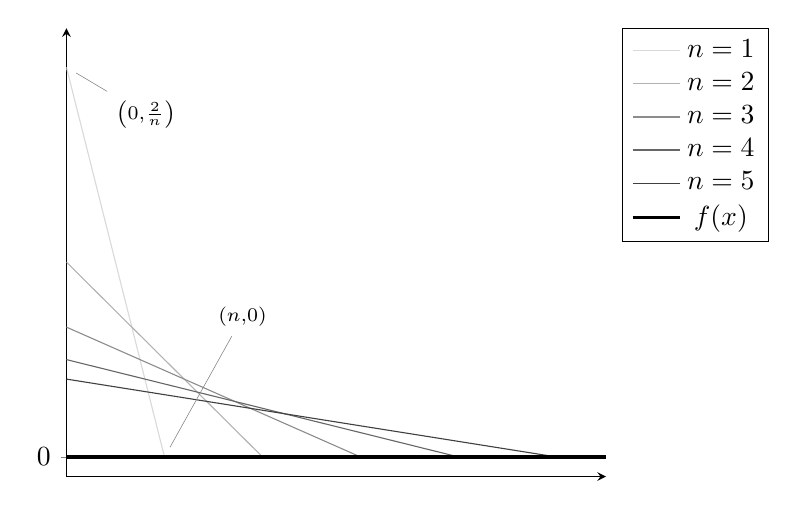
\begin{tikzpicture}
		\begin{axis}[
						enlargelimits,
						legend pos=outer north east,
						axis x line=bottom,axis y line=middle,
						xmin=0,xmax=5.5,ymin=-0.1,ymax=2.2,ytick={0},xtick=\empty
					]
			\addplot [color=black!15!white] coordinates {(0,2/1) (1,0)};
			\addplot [color=black!30!white] coordinates {(0,2/2) (2,0)};
			\addplot [color=black!45!white] coordinates {(0,2/3) (3,0)};
			\addplot [color=black!60!white] coordinates {(0,2/4) (4,0)};
			\addplot [color=black!75!white] coordinates {(0,2/5) (5,0)};
			\addplot [very thick,color=black,domain=0:5.5]  {0};
			\node [pin=-30:{$\scriptstyle\left(0,\frac2{n}\right)$}] at (axis cs:0,2) {};
			\node [pin={[pin distance=1.5 cm]70:{$\scriptstyle(n,0)$}}] at (axis cs:1,0) {};
			\legend{$n=1$,$n=2$,$n=3$,$n=4$,$n=5$,$f(x)$}
		\end{axis}
	\end{tikzpicture}
	\caption{La successione $f_n(x)=\frac2{n}-\frac2{n^2}x$ per $x<n$ e $f_n(x)=0$ per $x\geq n$ forma un triangolo di area 1 con gli assi cartesiani, indipendentemente dal valore di $n$.}
	\label{fig:succ_integrazione_illimitata}
\end{figure}
